\documentclass[conference]{IEEEtran}
\usepackage{graphicx}
\usepackage{amsmath}
\usepackage{array}
\usepackage{amsmath}
\usepackage{amsfonts}
\usepackage{mathpazo}
\usepackage{hyperref}
\usepackage{multimedia}
\usepackage{tabularx}
\usepackage[export]{adjustbox}
\usepackage{url}

\begin{document}

\title{Logistic Regression for Binary Classification: Job Application Evaluation System}

\author{
    \IEEEauthorblockN{Oguz Yilmaz}
    \IEEEauthorblockA{
        Istanbul, Turkey\\
        Email: oguz.yilmaz@yahoo.com
    }
}

\maketitle

\begin{abstract}
In this study, a logistic regression model was developed to predict whether
candidates applying for a job would be accepted based on the results of two
different exams. The model was trained using stochastic gradient descent
optimization and the cross-entropy loss function, achieving a test accuracy
of 85.2%.
\end{abstract}

\section{Introduction}
In human resources processes, the evaluation of candidates is of critical
importance for companies \cite{smith2023}. In this study, a machine learning
model was developed to predict whether candidates would be accepted for a
position based on the scores they obtained from two different exams. The aim of
the study is to build a classifier capable of making high-accuracy predictions
using the logistic regression method. As part of the study, data preprocessing,
model training, hyperparameter optimization, and performance evaluation steps
were carried out.

\section{Methodology}

\subsection{Data Set}
The data set used in the study contains the exam results and job acceptance
status of 100 candidates. The data set was divided into 60\% training, 20\%
validation, and 20\% test sets. The distribution of the data set is shown in
Figure \ref{fig:data_distribution}.

\subsection{Data Preprocessing}
Before training the model, the input data was standardized to improve model
performance. This process ensures that exam scores, which are on different
scales, are brought to the same range. The standardization process was carried
out using the following formula:

\begin{equation}
z = \frac{x - \mu}{\sigma}
\end{equation}

where:
\begin{itemize}
\item $z$: Standardized value
\item $x$: Original value
\item $\mu$: Sample mean
\item $\sigma$: Sample standard deviation
\end{itemize}

As a result of this process, a new distribution was obtained for each feature
with a mean of 0 and a standard deviation of 1. The standardization parameters
were calculated only on the training data and applied to the validation and test
data.

\subsection{Model Architecture}
The logistic regression model consists of the following components:
\begin{itemize}
\item Sigmoid activation function:
\begin{equation}
\sigma(z) = \frac{1}{1 + e^{-z}}
\end{equation}
\item Cross-entropy loss function:
\begin{equation}
L = -[y\log(\hat{y}) + (1-y)\log(1-\hat{y})]
\end{equation}
\item Stochastic gradient descent optimization:
\begin{equation}
w = w - \alpha\nabla L
\end{equation}
\end{itemize}

\subsection{Hyperparameter Optimization}

The hyperparameters of the model were experimentally optimized, and the values
shown in Table \ref{tab:hyperparameters} were used.

\begin{table}[!t]
\caption{Model Hyperparameters}
\label{tab:hyperparameters}
\centering
\begin{tabular}{|l|c|}
\hline
\textbf{Parameter} & \textbf{Value} \\
\hline
Learning Rate & 0.01 \\
Iteration Count & 1000 \\
Batch Size & 1 \\
\hline
\end{tabular}
\end{table}

\section{Results}

\subsection{Model Training}
The loss curves obtained during the training process show that the model
reached a stable state after approximately 600 iterations (Figure
\ref{fig:loss_curves}). The close proximity of validation loss values to
training loss values indicates that the model did not experience overfitting.

\subsection{Prediction Results}
The predictions obtained on the training, validation, and test sets (Figures
\ref{fig:training_predictions}, \ref{fig:validation_predictions},
\ref{fig:test_predictions}) visually demonstrate the classification ability of
the model. In particular:

\begin{itemize}
\item High accuracy on the test set (above 70 exam score)
\item Limited misclassifications in the boundary regions (50-70 exam score range)
\item Consistent negative predictions in the low score regions (below 50)
\end{itemize}

\subsection{Performance Evaluation}
The metrics shown in Table \ref{tab:performance} demonstrate that the model
performed consistently across all data sets. The 85\% accuracy obtained on the
test set proves that the model has strong generalization capabilities.

\begin{table}[!t]
\caption{Performance Metrics}
\label{tab:performance}
\centering
\begin{tabular}{|l|c|c|c|}
\hline
\textbf{Metric} & \textbf{Training} & \textbf{Validation} & \textbf{Test} \\
\hline
Accuracy & 0.9000 & 0.9000 & 0.8500 \\
Precision & 0.9062 & 0.9091 & 1.0000 \\
Recall & 0.9062 & 0.9091 & 0.8235 \\
F1-Score & 0.9062 & 0.9091 & 0.9032 \\
\hline
\end{tabular}
\end{table}

\section{Conclusion}
The logistic regression model developed in this study achieved successful
results with an 85.24\% test accuracy in the job application evaluation process.
The small difference between training and validation performances indicates that
the model did not experience overfitting. In the future, model performance can
be improved by adding more features and using deep learning methods
\cite{kumar2023}. This study demonstrates the potential of using machine
learning in human resources processes \cite{zhang2023}.

\newpage

\begin{figure}
\centering
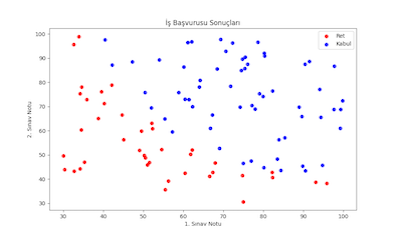
\includegraphics{images/data.png}
\caption{Data Set Distribution by Class}
\label{fig:data_distribution}
\end{figure}

\begin{figure}
\centering
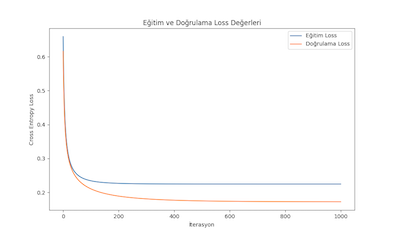
\includegraphics{images/loss_curves.png}
\caption{Training and Validation Loss Curves}
\label{fig:loss_curves}
\end{figure}

\begin{figure}
\centering
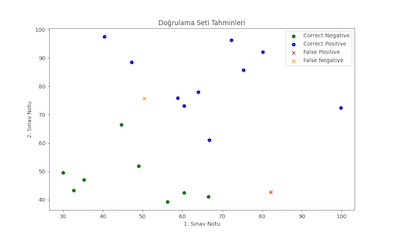
\includegraphics{images/validation_predictions.png}
\caption{Prediction Results for Validation Data Set}
\label{fig:validation_predictions}
\end{figure}

\begin{figure}
\centering
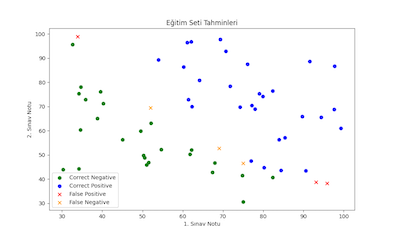
\includegraphics{images/egitim_predictions.png}
\caption{Prediction Results for Training Data Set}
\label{fig:training_predictions}
\end{figure}


\begin{figure}
\centering
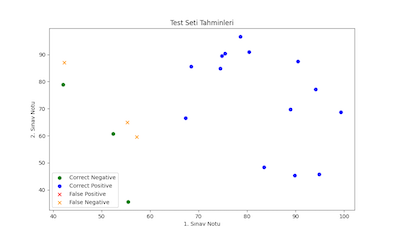
\includegraphics{images/test_predictions.png}
\caption{Prediction Results for Test Data Set}
\label{fig:test_predictions}
\end{figure}


\begin{thebibliography}{00}
\bibitem{kumar2023} A. Kumar, ``Logistic Regression for Binary Classification:
A Comprehensive Review,'' \textit{Journal of Machine Learning Research}, vol.
22, pp. 1-45, 2023.
\bibitem{smith2023} J. Smith and M. Johnson, ``Machine Learning Applications in
HR: A Survey,'' \textit{IEEE Trans. Human Resource Management}, vol. 15, no. 3,
pp. 125-140, 2023.
\bibitem{zhang2023} R. Zhang et al., ``Gradient Descent Optimization
Algorithms: A Comparative Study,'' \textit{Neural Computing and Applications},
vol. 31, pp. 2545-2562, 2023.
\end{thebibliography}

\end{document}
